\documentclass[12pt,a4paper]{article}
\usepackage[UTF8]{ctex}
\usepackage{amsmath,amssymb}
\usepackage{geometry}
\usepackage{hyperref}
\usepackage{tikz}
\usetikzlibrary{shapes.geometric, arrows.meta, positioning, fit, backgrounds, calc}

\geometry{margin=2.5cm}

\title{Torus网格切割项目：函数调用流程图（现行版本）}
\author{}
\date{\today}

\begin{document}

\maketitle

\section{整体架构流程图}

\begin{figure}[h]
\centering
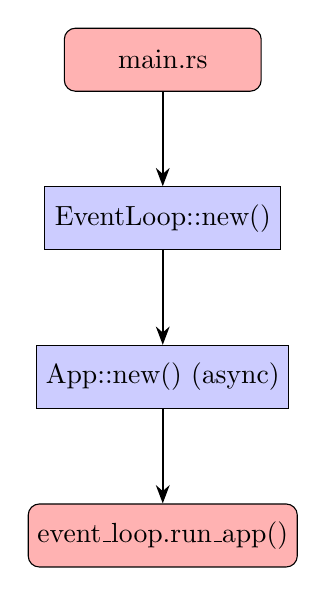
\begin{tikzpicture}[
    node distance=1.2cm,
    startstop/.style={rectangle, rounded corners, minimum width=2.5cm, minimum height=0.8cm, text centered, draw=black, fill=red!30},
    process/.style={rectangle, minimum width=3cm, minimum height=0.8cm, text centered, draw=black, fill=blue!20},
    decision/.style={diamond, minimum width=2cm, minimum height=0.8cm, text centered, draw=black, fill=green!20, aspect=2},
    io/.style={trapezium, trapezium left angle=70, trapezium right angle=110, minimum width=2cm, minimum height=0.8cm, text centered, draw=black, fill=yellow!20},
    arrow/.style={thick,->,>=Stealth},
    module/.style={rectangle, rounded corners, minimum width=4cm, minimum height=0.6cm, text centered, draw=black, fill=orange!30},
]

    % Main entry
    \node (main) [startstop] {main.rs};
    \node (event_loop) [process, below=of main] {EventLoop::new()};
    \node (app_new) [process, below=of event_loop] {App::new() (async)};
    \node (run_app) [startstop, below=of app_new] {event\_loop.run\_app()};

    \draw [arrow] (main) -- (event_loop);
    \draw [arrow] (event_loop) -- (app_new);
    \draw [arrow] (app_new) -- (run_app);

\end{tikzpicture}
\caption{程序入口流程}
\end{figure}

\section{App 初始化流程}

\begin{figure}[h]
\centering
\begin{tikzpicture}[
    node distance=1cm,
    startstop/.style={rectangle, rounded corners, minimum width=2.5cm, minimum height=0.8cm, text centered, draw=black, fill=red!30},
    process/.style={rectangle, minimum width=3.5cm, minimum height=0.8cm, text centered, draw=black, fill=blue!20},
    module/.style={rectangle, rounded corners, minimum width=4cm, minimum height=0.6cm, text centered, draw=black, fill=orange!30},
    arrow/.style={thick,->,>=Stealth},
]

    % resumed event
    \node (resumed) [startstop] {resumed() 事件触发};
    \node (init_wgpu) [module, below=of resumed] {init\_gpu()};
    \node (wgpu_device) [process, below left=0.8cm and 0.5cm of init_wgpu] {wgpu::Device};
    \node (wgpu_queue) [process, below=0.8cm of init_wgpu] {wgpu::Queue};
    \node (wgpu_surface) [process, below right=0.8cm and 0.5cm of init_wgpu] {wgpu::Surface};

    \node (create_shader) [module, below=2cm of init_wgpu] {create\_shader\_module()};
    \node (mesh_shader) [process, below left=0.8cm and 0.5cm of create_shader] {mesh.wgsl};
    \node (wf_shader) [process, below right=0.8cm and 0.5cm of create_shader] {wireframe.wgsl};

    \node (egui_init) [module, below=2cm of create_shader] {egui\_wgpu::Renderer::new()};

    \node (build_mesh) [startstop, below=of egui_init] {build\_torus\_mesh()};
    \node (rebuild) [startstop, below=of build_mesh] {rebuild\_render\_state()};

    \draw [arrow] (resumed) -- (init_wgpu);
    \draw [arrow] (init_wgpu) -- (wgpu_device);
    \draw [arrow] (init_wgpu) -- (wgpu_queue);
    \draw [arrow] (init_wgpu) -- (wgpu_surface);
    \draw [arrow] (init_wgpu) -- (create_shader);
    \draw [arrow] (create_shader) -- (mesh_shader);
    \draw [arrow] (create_shader) -- (wf_shader);
    \draw [arrow] (create_shader) -- (egui_init);
    \draw [arrow] (egui_init) -- (build_mesh);
    \draw [arrow] (build_mesh) -- (rebuild);

\end{tikzpicture}
\caption{App 初始化流程（App::new 为 async；GPU/着色器/egui 在 resumed 中创建）}
\end{figure}

\section{Torus 网格构建流程}

\begin{figure}[h]
\centering
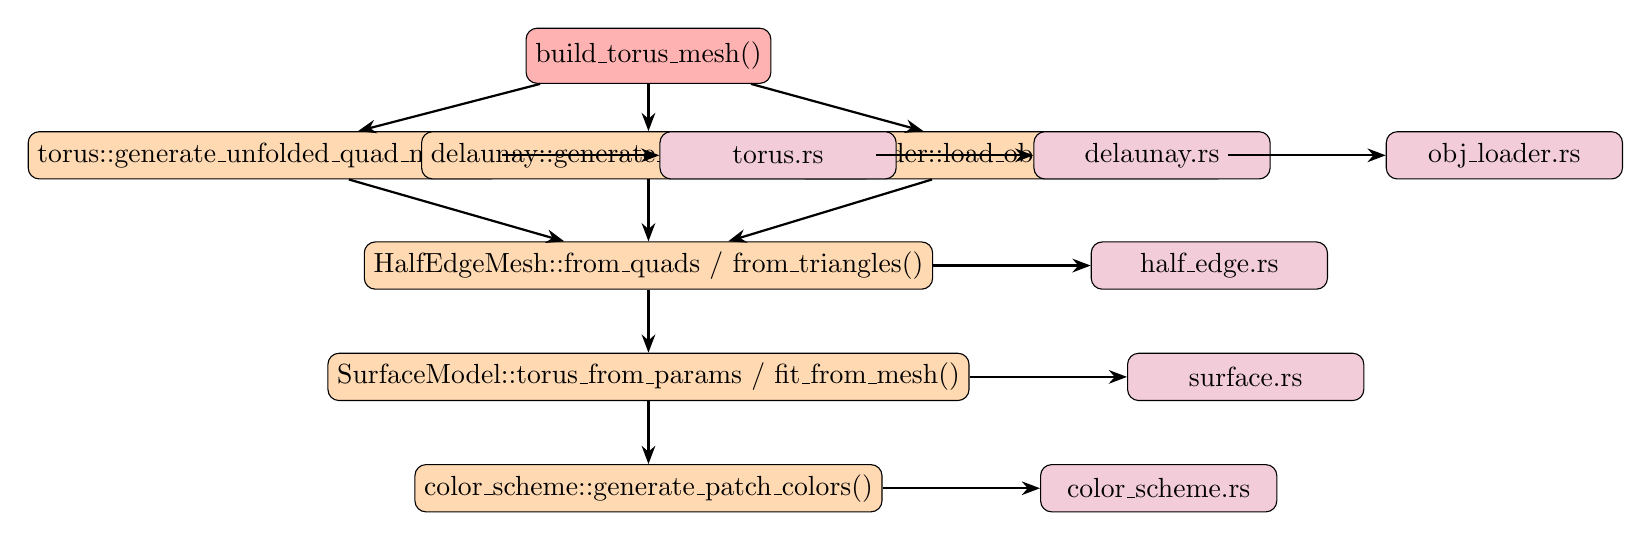
\begin{tikzpicture}[
    node distance=0.8cm,
    startstop/.style={rectangle, rounded corners, minimum width=2.5cm, minimum height=0.7cm, text centered, draw=black, fill=red!30},
    process/.style={rectangle, minimum width=4cm, minimum height=0.7cm, text centered, draw=black, fill=blue!20},
    module/.style={rectangle, rounded corners, minimum width=4.5cm, minimum height=0.6cm, text centered, draw=black, fill=orange!30},
    file/.style={rectangle, rounded corners, minimum width=3cm, minimum height=0.6cm, text centered, draw=black, fill=purple!20},
    arrow/.style={thick,->,>=Stealth},
]

    % build_torus_mesh
    \node (build_mesh) [startstop] {build\_torus\_mesh()};

    % mesh source dispatch
    \node (src_quad) [module, below left=0.6cm and 0.3cm of build_mesh]
      {torus::generate\_unfolded\_quad\_mesh()};
    \node (src_del) [module, below=0.6cm of build_mesh]
      {delaunay::generate\_delaunay\_mesh()};
    \node (src_obj) [module, below right=0.6cm and 0.3cm of build_mesh]
      {obj\_loader::load\_obj\_as\_half\_edge()};

    \node (quad_file) [file, right=2cm of src_quad] {torus.rs};
    \node (del_file) [file, right=2cm of src_del] {delaunay.rs};
    \node (obj_file) [file, right=2cm of src_obj] {obj\_loader.rs};

    % half-edge construction
    \node (from_he) [module, below=2.0cm of build_mesh]
      {HalfEdgeMesh::from\_quads / from\_triangles()};
    \node (he_file) [file, right=2cm of from_he] {half\_edge.rs};

    % surface model
    \node (surf) [module, below=of from_he] {SurfaceModel::torus\_from\_params / fit\_from\_mesh()};
    \node (surf_file) [file, right=2cm of surf] {surface.rs};

    % color
    \node (gen_color) [module, below=of surf] {color\_scheme::generate\_patch\_colors()};
    \node (color_file) [file, right=2cm of gen_color] {color\_scheme.rs};

    \draw [arrow] (build_mesh) -- (src_quad);
    \draw [arrow] (build_mesh) -- (src_del);
    \draw [arrow] (build_mesh) -- (src_obj);
    \draw [arrow] (src_quad) -- (quad_file);
    \draw [arrow] (src_del) -- (del_file);
    \draw [arrow] (src_obj) -- (obj_file);
    \draw [arrow] (src_quad) -- (from_he);
    \draw [arrow] (src_del) -- (from_he);
    \draw [arrow] (src_obj) -- (from_he);
    \draw [arrow] (from_he) -- (he_file);
    \draw [arrow] (from_he) -- (surf);
    \draw [arrow] (surf) -- (surf_file);
    \draw [arrow] (surf) -- (gen_color);
    \draw [arrow] (gen_color) -- (color_file);

\end{tikzpicture}
\caption{Torus 网格构建流程（Quad / Delaunay / OBJ 三源）}
\end{figure}

\section{切割与补片分配流程}

\begin{figure}[h]
\centering
\begin{tikzpicture}[
    node distance=0.8cm,
    startstop/.style={rectangle, rounded corners, minimum width=2.5cm, minimum height=0.7cm, text centered, draw=black, fill=red!30},
    process/.style={rectangle, minimum width=4cm, minimum height=0.7cm, text centered, draw=black, fill=blue!20},
    module/.style={rectangle, rounded corners, minimum width=4.5cm, minimum height=0.6cm, text centered, draw=black, fill=orange!30},
    file/.style={rectangle, rounded corners, minimum width=3cm, minimum height=0.6cm, text centered, draw=black, fill=purple!20},
    decision/.style={diamond, minimum width=2.2cm, minimum height=0.7cm, text centered, draw=black, fill=green!20, aspect=2},
    arrow/.style={thick,->,>=Stealth},
]

    \node (reapply) [startstop] {reapply\_cuts()};

    \node (cutmode) [decision, below=of reapply] {cut\_mode?};
    \node (grid_cut) [module, below left=1.0cm and 0.3cm of cutmode]
      {cut\_mesh\_by\_grid(u\_vals, v\_vals)};
    \node (knot_cut) [module, below right=1.0cm and 0.3cm of cutmode]
      {cut\_mesh\_by\_knots(k\_values)};

    \node (cut_file) [file, right=2cm of grid_cut] {cut.rs};
    \node (knot_file) [file, right=2cm of knot_cut] {cut.rs};

    \node (intersect_u) [process, below left=0.6cm and 0.3cm of grid_cut]
      {intersect\_face\_u / intersect\_face\_v};
    \node (intersect_k) [process, below right=0.6cm and 0.3cm of knot_cut]
      {intersect\_face\_knot\_branch (多分支)};

    \node (split_edge) [process, below=1.6cm of cutmode] {split\_edge() + split\_face()};
    \node (triang) [process, below=of split_edge] {triangulate\_face()（局部）};

    \node (assign) [module, below=of triang] {assign\_patch\_indices / assign\_multi\_knot\_patch\_indices};
    \node (assign_file) [file, right=2cm of assign] {cut.rs};

    \draw [arrow] (reapply) -- (cutmode);
    \draw [arrow] (cutmode) -- node[left] {Grid} (grid_cut);
    \draw [arrow] (cutmode) -- node[right] {Knot} (knot_cut);
    \draw [arrow] (grid_cut) -- (cut_file);
    \draw [arrow] (knot_cut) -- (knot_file);
    \draw [arrow] (grid_cut) -- (intersect_u);
    \draw [arrow] (knot_cut) -- (intersect_k);
    \draw [arrow] (intersect_u) -- (split_edge);
    \draw [arrow] (intersect_k) -- (split_edge);
    \draw [arrow] (split_edge) -- (triang);
    \draw [arrow] (triang) -- (assign);
    \draw [arrow] (assign) -- (assign_file);

\end{tikzpicture}
\caption{切割与补片分配流程（Grid / Knot 两种模式）}
\end{figure}

\section{渲染状态构建流程}

\begin{figure}[h]
\centering
\begin{tikzpicture}[
    node distance=0.8cm,
    startstop/.style={rectangle, rounded corners, minimum width=2.5cm, minimum height=0.7cm, text centered, draw=black, fill=red!30},
    process/.style={rectangle, minimum width=3.5cm, minimum height=0.7cm, text centered, draw=black, fill=blue!20},
    module/.style={rectangle, rounded corners, minimum width=4cm, minimum height=0.6cm, text centered, draw=black, fill=orange!30},
    file/.style={rectangle, rounded corners, minimum width=2.5cm, minimum height=0.6cm, text centered, draw=black, fill=purple!20},
    arrow/.style={thick,->,>=Stealth},
]

    % rebuild_render_state
    \node (rebuild) [startstop] {rebuild\_render\_state()};

    \node (to_view) [process, below=of rebuild] {to\_view\_mesh()（3D / UV 平面）};
    \node (collect) [process, below=of to_view] {遍历有效面 → GpuVertex[]};

    \node (rs_new) [module, below=of collect] {RenderState::new / update\_mesh\_buffers()};
    \node (state_file) [file, right=2cm of rs_new] {state.rs};

    \node (create_pipe) [module, below left=0.6cm and 0.3cm of rs_new] {create\_mesh\_pipeline()};
    \node (pipe_file) [file, below=0.6cm of create_pipe] {pipeline.rs};

    \node (upload_mesh) [module, below=0.6cm of rs_new] {mesh\_buffer.rs};
    \node (create_wf) [module, below right=0.6cm and 0.3cm of rs_new] {wireframe.rs};

    \draw [arrow] (rebuild) -- (to_view);
    \draw [arrow] (to_view) -- (collect);
    \draw [arrow] (collect) -- (rs_new);
    \draw [arrow] (rs_new) -- (state_file);
    \draw [arrow] (rs_new) -- (create_pipe);
    \draw [arrow] (create_pipe) -- (pipe_file);
    \draw [arrow] (rs_new) -- (upload_mesh);
    \draw [arrow] (rs_new) -- (create_wf);

\end{tikzpicture}
\caption{渲染状态构建流程}
\end{figure}

\section{渲染循环流程}

\begin{figure}[h]
\centering
\begin{tikzpicture}[
    node distance=0.7cm,
    startstop/.style={rectangle, rounded corners, minimum width=2.5cm, minimum height=0.7cm, text centered, draw=black, fill=red!30},
    process/.style={rectangle, minimum width=3cm, minimum height=0.7cm, text centered, draw=black, fill=blue!20},
    decision/.style={diamond, minimum width=1.5cm, minimum height=0.6cm, text centered, draw=black, fill=green!20, aspect=2.5},
    module/.style={rectangle, rounded corners, minimum width=3.5cm, minimum height=0.6cm, text centered, draw=black, fill=orange!30},
    arrow/.style={thick,->,>=Stealth},
]

    % render entry
    \node (render) [startstop] {render()};

    \node (update) [process, below=of render] {update()（相机键盘）};
    \node (ui_panel) [module, below=of update] {panel::render\_ui\_panel()};

    \node (dec_rebuild) [decision, below=of ui_panel] {rebuild?};
    \node (dec_export) [decision, below left=0.6cm and 0.3cm of dec_rebuild] {export?};

    \node (rebuild_mesh) [process, below=of dec_rebuild] {build\_torus\_mesh() + reapply\_cuts()};
    \node (export_mesh) [module, below=of dec_export] {export::export\_mesh / export\_by\_patch};

    \node (mesh_pass) [process, below=1.5cm of rebuild_mesh] {Mesh Pass};
    \node (wf_dec) [decision, below=of mesh_pass] {show edges?};
    \node (wf_pass) [process, below=of wf_dec] {Edge / Wireframe Pass};
    \node (egui_pass) [process, below=of wf_pass] {egui Overlay Pass};
    \node (present) [startstop, below=of egui_pass] {output.present()};

    \draw [arrow] (render) -- (update);
    \draw [arrow] (update) -- (ui_panel);
    \draw [arrow] (ui_panel) -- (dec_rebuild);
    \draw [arrow] (dec_rebuild) -- node[right] {yes} (rebuild_mesh);
    \draw [arrow] (dec_rebuild) -- (dec_export);
    \draw [arrow] (dec_export) -- node[right] {yes} (export_mesh);
    \draw [arrow] (rebuild_mesh) -- (mesh_pass);
    \draw [arrow] (mesh_pass) -- (wf_dec);
    \draw [arrow] (wf_dec) -- node[right] {yes} (wf_pass);
    \draw [arrow] (wf_pass) -- (egui_pass);
    \draw [arrow] (egui_pass) -- (present);

\end{tikzpicture}
\caption{渲染循环流程}
\end{figure}

\section{UI 面板详细流程}

\begin{figure}[h]
\centering
\begin{tikzpicture}[
    node distance=0.5cm,
    startstop/.style={rectangle, rounded corners, minimum width=2.5cm, minimum height=0.6cm, text centered, draw=black, fill=red!30},
    process/.style={rectangle, minimum width=3cm, minimum height=0.6cm, text centered, draw=black, fill=blue!20},
    input/.style={rectangle, minimum width=2.8cm, minimum height=0.6cm, text centered, draw=black, fill=cyan!20},
    decision/.style={diamond, minimum width=1.2cm, minimum height=0.5cm, text centered, draw=black, fill=green!20, aspect=2.5},
    label/.style={rectangle, rounded corners, minimum width=2cm, minimum height=0.5cm, text centered, draw=black, fill=yellow!30},
    arrow/.style={thick,->,>=Stealth},
]

    % Panel entry
    \node (panel) [startstop] {render\_ui\_panel()};

    % Left tabs
    \node (tabs) [process, below=of panel] {4 Tabs: Mesh / Cut / Shader / Export};

    % Mesh tab
    \node (mesh_tab) [label, below=of tabs] {"1. Mesh"};
    \node (mesh_src) [input, below=of mesh_tab] {Radio: Quad / Delaunay / OBJ};
    \node (res_u) [input, below=of mesh_src] {Slider: U divisions (res\_u)};
    \node (res_v) [input, below=of res_v] {Slider: V divisions (res\_v) / Point count};
    \node (major_r) [input, below=of res_u] {Slider: Major Radius (R)};
    \node (minor_r) [input, below=of major_r] {Slider: Minor Radius (r)};
    \node (rebuild_btn) [process, below=of minor_r] {action.rebuild = true};

    % Cut tab
    \node (cut_tab) [label, below=1cm of rebuild_btn] {"2. Cut"};
    \node (cut_mode) [input, below=of cut_tab] {Select: Grid / Knot};
    \node (grid_loops) [input, below=of cut_mode] {Sliders: U-Loops / V-Loops};
    \node (knot_k) [input, below=of grid_loops] {Checkbox+Drag: k1 / k2 (Cut)};
    \node (reapply_btn) [process, below=of knot_k] {action.reapply\_cuts = true};

    % Shader tab
    \node (shader_tab) [label, below=1cm of reapply_btn] {"3. Shader"};
    \node (patch_vis) [input, below=of shader_tab] {Patch visibility / material};
    \node (per_patch) [input, below=of patch_vis] {Per-patch shader override};
    \node (apply_btn) [process, below=of per_patch] {action.apply\_patch\_shaders / recolor};

    % Export tab
    \node (export_tab) [label, below=1cm of apply_btn] {"4. Export"};
    \node (fmt) [input, below=of export_tab] {ComboBox: OBJ / STL / PLY};
    \node (export_path) [input, below=of fmt] {TextEdit: path / dir};
    \node (export_btn) [process, below=of export_path] {Button: Export → action.export};

    % Right panel
    \node (disp_panel) [label, right=1.5cm of tabs] {"Display Settings"};
    \node (view_mode) [input, right=1.5cm of mesh_tab] {View: 3D / Planar UV};
    \node (lighting) [input, right=1.5cm of res_u] {Lighting / AO};
    \node (edges) [input, right=1.5cm of major_r] {Show mesh/cut edges};
    \node (shader_combo) [input, right=1.5cm of minor_r] {Global shader + params};
    \node (color_mode) [input, right=1.5cm of rebuild_btn] {Color: Solid / ByRegion};
    \node (scheme) [input, right=1.5cm of cut_tab] {ColorScheme: Rainbow/…};
    \node (stats) [input, right=1.5cm of grid_loops] {Mesh info (verts/faces/…)};

    % Return
    \node (return) [startstop, below=of export_btn] {return UiAction};

    \draw [arrow] (panel) -- (tabs);
    \draw [arrow] (tabs) -- (mesh_tab);
    \draw [arrow] (mesh_tab) -- (mesh_src);
    \draw [arrow] (mesh_src) -- (res_u);
    \draw [arrow] (res_u) -- (res_v);
    \draw [arrow] (res_u) -- (major_r);
    \draw [arrow] (major_r) -- (minor_r);
    \draw [arrow] (minor_r) -- (rebuild_btn);

    \draw [arrow] (rebuild_btn) -- (cut_tab);
    \draw [arrow] (cut_tab) -- (cut_mode);
    \draw [arrow] (cut_mode) -- (grid_loops);
    \draw [arrow] (grid_loops) -- (knot_k);
    \draw [arrow] (knot_k) -- (reapply_btn);

    \draw [arrow] (reapply_btn) -- (shader_tab);
    \draw [arrow] (shader_tab) -- (patch_vis);
    \draw [arrow] (patch_vis) -- (per_patch);
    \draw [arrow] (per_patch) -- (apply_btn);

    \draw [arrow] (apply_btn) -- (export_tab);
    \draw [arrow] (export_tab) -- (fmt);
    \draw [arrow] (fmt) -- (export_path);
    \draw [arrow] (export_path) -- (export_btn);
    \draw [arrow] (export_btn) -- (return);

    \draw [arrow] (tabs) -- (disp_panel);
    \draw [arrow] (disp_panel) -- (view_mode);
    \draw [arrow] (view_mode) -- (lighting);
    \draw [arrow] (lighting) -- (edges);
    \draw [arrow] (edges) -- (shader_combo);
    \draw [arrow] (shader_combo) -- (color_mode);
    \draw [arrow] (color_mode) -- (scheme);
    \draw [arrow] (scheme) -- (stats);

\end{tikzpicture}
\caption{UI 面板详细流程（4 个 Tab + 右侧常驻显示面板）}
\end{figure}

\section{导出流程}

\begin{figure}[h]
\centering
\begin{tikzpicture}[
    node distance=0.8cm,
    startstop/.style={rectangle, rounded corners, minimum width=2.5cm, minimum height=0.7cm, text centered, draw=black, fill=red!30},
    process/.style={rectangle, minimum width=3cm, minimum height=0.7cm, text centered, draw=black, fill=blue!20},
    module/.style={rectangle, rounded corners, minimum width=3.5cm, minimum height=0.6cm, text centered, draw=black, fill=orange!30},
    file/.style={rectangle, rounded corners, minimum width=2.5cm, minimum height=0.6cm, text centered, draw=black, fill=purple!20},
    arrow/.style={thick,->,>=Stealth},
]

    % Export entry
    \node (export_action) [startstop] {action.export};
    \node (to_view) [process, below=of export_action] {to\_view\_mesh()（所见即所得）};
    \node (export_mesh) [module, below=of to_view] {export::export\_mesh()};
    \node (export_file) [file, right=2cm of export_mesh] {obj.rs / stl.rs / ply.rs};

    \node (write_header) [process, below=of export_mesh] {write header};
    \node (write_verts) [process, below=of write_header] {write vertices};
    \node (write_normals) [process, below=of write_verts] {compute/write normals (OBJ)};
    \node (write_faces) [process, below=of write_normals] {write faces};
    \node (out) [startstop, below=of write_faces] {torus\_cut.obj / .stl / .ply};

    \draw [arrow] (export_action) -- (to_view);
    \draw [arrow] (to_view) -- (export_mesh);
    \draw [arrow] (export_mesh) -- (export_file);
    \draw [arrow] (export_mesh) -- (write_header);
    \draw [arrow] (write_header) -- (write_verts);
    \draw [arrow] (write_verts) -- (write_normals);
    \draw [arrow] (write_normals) -- (write_faces);
    \draw [arrow] (write_faces) -- (out);

\end{tikzpicture}
\caption{导出流程（OBJ / STL / PLY，按 patch 时每片一个文件）}
\end{figure}

\section{模块依赖关系图}

\begin{figure}[h]
\centering
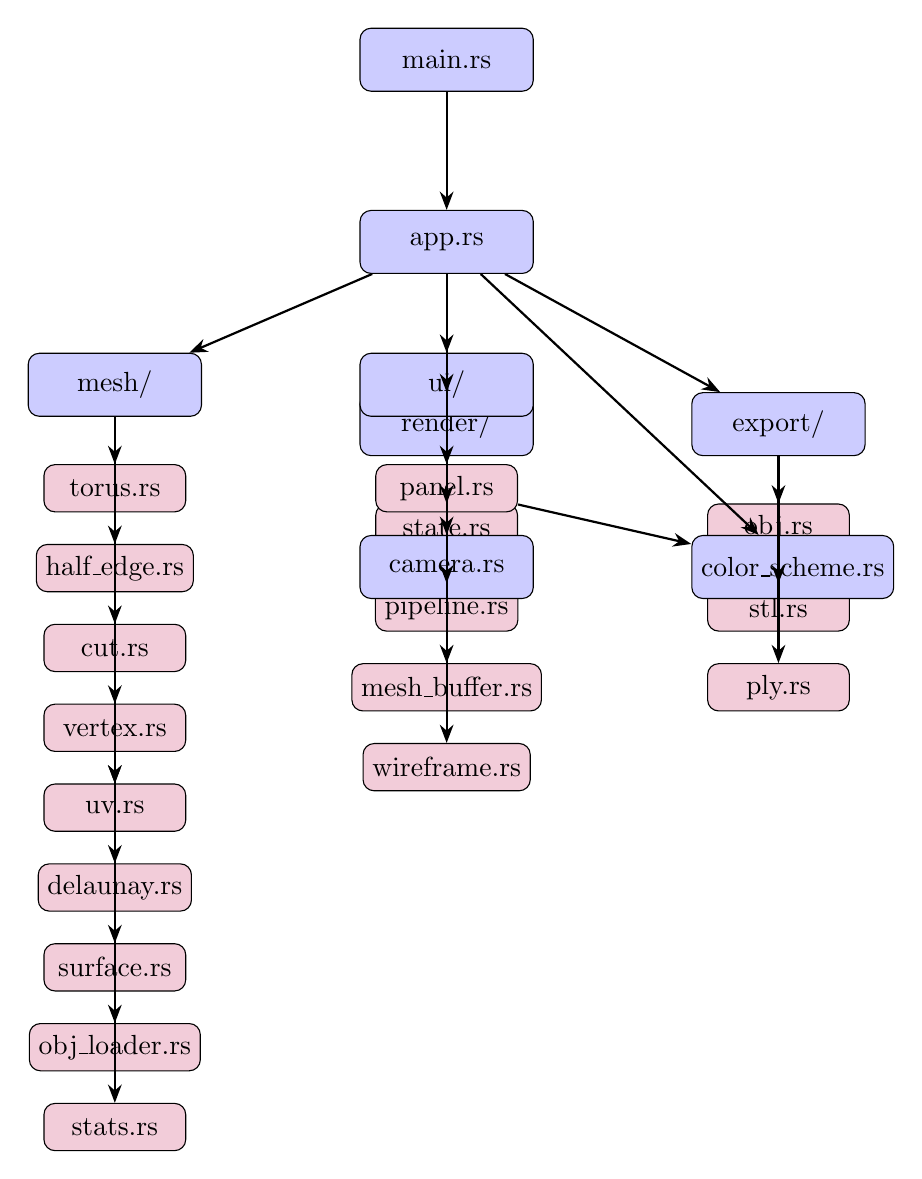
\begin{tikzpicture}[
    node distance=1.5cm,
    module/.style={rectangle, rounded corners, minimum width=2.2cm, minimum height=0.8cm, text centered, draw=black, fill=blue!20},
    file/.style={rectangle, rounded corners, minimum width=1.8cm, minimum height=0.6cm, text centered, draw=black, fill=purple!20},
    arrow/.style={thick,->,>=Stealth},
]

    % Core modules
    \node (main) [module] {main.rs};
    \node (app) [module, below=of main] {app.rs};

    % Mesh modules
    \node (mesh) [module, below left=1cm and 2cm of app] {mesh/};
    \node (torus) [file, below=0.6cm of mesh] {torus.rs};
    \node (half_edge) [file, below=0.4cm of torus] {half\_edge.rs};
    \node (cut) [file, below=0.4cm of half_edge] {cut.rs};
    \node (vertex) [file, below=0.4cm of cut] {vertex.rs};
    \node (uv) [file, below=0.4cm of vertex] {uv.rs};
    \node (delaunay) [file, below=0.4cm of uv] {delaunay.rs};
    \node (surface) [file, below=0.4cm of delaunay] {surface.rs};
    \node (obj_loader) [file, below=0.4cm of surface] {obj\_loader.rs};
    \node (stats) [file, below=0.4cm of obj_loader] {stats.rs};

    % Render modules
    \node (render) [module, below=of app] {render/};
    \node (state) [file, below=0.6cm of render] {state.rs};
    \node (pipeline) [file, below=0.4cm of state] {pipeline.rs};
    \node (mesh_buf) [file, below=0.4cm of pipeline] {mesh\_buffer.rs};
    \node (wireframe) [file, below=0.4cm of mesh_buf] {wireframe.rs};

    % Other modules
    \node (export) [module, right=2cm of render] {export/};
    \node (obj) [file, below=0.6cm of export] {obj.rs};
    \node (stl) [file, below=0.4cm of obj] {stl.rs};
    \node (ply) [file, below=0.4cm of stl] {ply.rs};

    \node (ui) [module, right=2cm of mesh] {ui/};
    \node (panel) [file, below=0.6cm of ui] {panel.rs};

    \node (camera) [module, below=1cm of render] {camera.rs};
    \node (color) [module, right=2cm of camera] {color\_scheme.rs};

    % Dependencies
    \draw [arrow] (main) -- (app);
    \draw [arrow] (app) -- (mesh);
    \draw [arrow] (app) -- (render);
    \draw [arrow] (app) -- (export);
    \draw [arrow] (app) -- (ui);
    \draw [arrow] (app) -- (camera);
    \draw [arrow] (app) -- (color);

    \draw [arrow] (mesh) -- (torus);
    \draw [arrow] (mesh) -- (half_edge);
    \draw [arrow] (mesh) -- (cut);
    \draw [arrow] (mesh) -- (vertex);
    \draw [arrow] (mesh) -- (uv);
    \draw [arrow] (mesh) -- (delaunay);
    \draw [arrow] (mesh) -- (surface);
    \draw [arrow] (mesh) -- (obj_loader);
    \draw [arrow] (mesh) -- (stats);

    \draw [arrow] (render) -- (state);
    \draw [arrow] (render) -- (pipeline);
    \draw [arrow] (render) -- (mesh_buf);
    \draw [arrow] (render) -- (wireframe);

    \draw [arrow] (export) -- (obj);
    \draw [arrow] (export) -- (stl);
    \draw [arrow] (export) -- (ply);
    \draw [arrow] (ui) -- (panel);

    \draw [arrow] (cut) -- (uv);
    \draw [arrow] (panel) -- (color);

\end{tikzpicture}
\caption{模块依赖关系图（现行：无 grid\_lines.rs / off.rs）}
\end{figure}

\section{关键数据流}

\begin{figure}[h]
\centering
\begin{tikzpicture}[
    node distance=1cm,
    data/.style={rectangle, rounded corners, minimum width=3cm, minimum height=0.7cm, text centered, draw=black, fill=cyan!20},
    process/.style={rectangle, minimum width=3.5cm, minimum height=0.7cm, text centered, draw=black, fill=blue!20},
    arrow/.style={thick,->,>=Stealth},
]

    \node (params) [data] {Torus 参数 (R, r, res\_u, res\_v)};
    \node (gen) [process, below=of params] {generate\_unfolded\_quad\_mesh / delaunay / load\_obj};
    \node (verts) [data, below=of gen] {positions + uvs + (quads|tris)};
    \node (he_build) [process, below=of verts] {HalfEdgeMesh::from\_quads / from\_triangles};
    \node (he_mesh) [data, below=of he_build] {HalfEdgeMesh};
    \node (cut) [process, below=of he_mesh] {cut\_mesh\_by\_grid / by\_knots};
    \node (cut_mesh) [data, below=of cut] {切割后的 HalfEdgeMesh};
    \node (assign) [process, below=of cut_mesh] {assign\_patch\_indices / multi\_knot};
    \node (gpu_data) [data, below=of assign] {GpuVertex[] + indices};
    \node (render) [process, below=of gpu_data] {wgpu 渲染管线};
    \node (image) [data, below=of render] {屏幕图像};

    \draw [arrow] (params) -- (gen);
    \draw [arrow] (gen) -- (verts);
    \draw [arrow] (verts) -- (he_build);
    \draw [arrow] (he_build) -- (he_mesh);
    \draw [arrow] (he_mesh) -- (cut);
    \draw [arrow] (cut) -- (cut_mesh);
    \draw [arrow] (cut_mesh) -- (assign);
    \draw [arrow] (assign) -- (gpu_data);
    \draw [arrow] (gpu_data) -- (render);
    \draw [arrow] (render) -- (image);

\end{tikzpicture}
\caption{关键数据流}
\end{figure}

\end{document}
